\documentclass[12pt]{article}

\usepackage{fullpage,url,amssymb,epsfig,color,xspace,enumerate,amsmath}
\usepackage[pdftitle={CS 240 Assignment 2},%
pdfsubject={University of Waterloo, CS 240, Spring 2014},%
pdfauthor={Alejandro Lopez-Ortiz}]{hyperref}
\usepackage{tikz}
\usetikzlibrary{shapes}

\renewcommand{\thesubsection}{Problem \arabic{subsection}}
\newcommand{\block}[4]{node[label=,rectangle split, rectangle split parts=#2](#3) {#4}}

\begin{document}

\begin{center}
{\Large\bf University of Waterloo}\\
\vspace{3mm}
{\Large\bf CS240 - Spring 2014}\\
\vspace{2mm}
{\Large\bf Assignment 4}\\
\vspace{3mm}
\textbf{Due Date: Wednesday July 9 at 09:15am}
\end{center}

\definecolor{care}{rgb}{0,0,0}
\def\question#1{\item[\bf #1.]}
\def\part#1{\item[\bf #1)]}
\newcommand{\pc}[1]{\mbox{\textbf{#1}}}

Please read
\url{http://www.student.cs.uwaterloo.ca/~cs240/s14/guidelines.pdf}
for guidelines on submission.

%%%%%%%%%%%%%%%%%%%%%%%%%%%%%%%%%%%%%%%%%%%%%%%%%%%%%%%%%%%%%
\subsection{[4+4+4+4 marks]}
\begin{enumerate}[(a)]
\item Give a recursive algorithm for finding the height of an arbitrary binary tree. Determine and
justify your algorithm's running time, using $O$-notation. Let this running time be $O(f(n))$.

\begin{verbatim}
  function maxHeight(node) {
    if(node = empty)
      return -1
    L = maxHeight(node.left)
    R = maxHeight(node.right)
    return max(L, R) + 1
  }
\end{verbatim}
This algorithm recursively checks the height of the children for each node (both of them, no matter whether those children are nodes or empty) and does one operation per call the running time for this algorithm is $O(2n)\in O(n)$.

Since we recurse on the left and right side we can say that we recurse on the left subtree T(l) where l is the number of nodes in the left subtree, and the right subtree which will be T(n-l-1) and we include the comparison made at the node, so +1.
\begin{align*}
  T(n) &= T(L) + T(n-L-1) + 1\\
  &< T(n -1) + T(n-n+1-1) + 1 \intertext{Since l must be less than n-1. }\\
  &= T(n -1) + T(0) + 1\\
  &= T(n-1) + 2\\
  &= T(n-2) + 2 + 2\\
  &= T(n - 3) + 6\\
  & \dots \\
  &= T(n-i) + 2i\\
  &\in O(2n)
\end{align*}

\item We want your bound above to be tight so give an example where your algorithm of part (a) takes time $\Omega(f(n))$.
Deduce then that the worst case running time is $\Theta(f(n))$.

Since the algorithm is called the same number of times no matter the shape of the tree we can say that the algorithm's time complexity is $\Omega(2n)\in \Omega(n)$. For example:

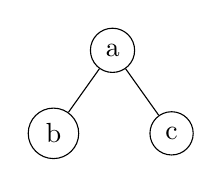
\begin{tikzpicture}[level distance=30pt,
      every node/.style={,circle,draw}]
      \node{a}
      child{
        node{b}
      }
      child{
        node{c}
      };
\end{tikzpicture}

Is completely equivalent to:

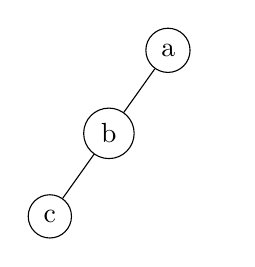
\begin{tikzpicture}[level distance=30pt,
      every node/.style={,circle,draw}]
      \node{a}
      child{
        node{b}
        child{
          node{c}
        }
        child{
          edge from parent[draw=none]
        }
      }
      child{
        edge from parent[draw=none]
      };
\end{tikzpicture}

Both of which have the time complexity of $\Omega(n)$

The worst case would be that L = 0 in the above equation.
\begin{align*}
      T(n) &= T(L) + T(n-L-1) + 1\\
        &= T(0) + T(n-1) + 1\\
        & \dots\\
        &= T(2n)\\
        &\in\Omega(n)
\end{align*}

So the time complexity is $\Theta(2n)\in\Theta(n)$
\item Give a recursive algorithm for finding the height of an AVL tree. Determine the running time
$O(g(n))$ of your algorithm, and show that $g(n) = o(f(n))$.

\begin{verbatim}
  function maxHeight(node) {
    if node = empty
      return -1
    if node.balance = -1
      return maxHeight(node.left) + 1
    if node.balance = 1
      return maxHeight(node.right) + 1
    else
      return maxHeight(node.left) + 1
  }
\end{verbatim}

If the node has is off balance we can know to iterate down the longer side, and if the node is balanced we know that both sides are of equal height so we can chose one at random, in this case the left side, to iterate down. Since this algorithm calls itself on one child no matter the balance of the node we can say that the worst case will be exactly the same as the best case and this will be equal to the height of the tree, which is $O(\log n)$. $\log n \in o(n)$  by the definition of little o.

\begin{align*}
    \intertext{Since the algorithm is called once per level }
    T(n) &= T(h-1) + 1\\
     &= T(h-2) + 2 \\
     & \dots\\
     &= \log n\\
     &\in O(\log n)\\
     &\in o(n)
\end{align*}

\item Give an example where your algorithm of part (c) takes time $\Omega(g(n))$. Deduce then that the worst case running time is $\Theta(g(n))$.

As stated above the algorithm is called once per layer of tree no matter what the balance of the node being iterated through so the best case is exactly the same as the worst case. For example:

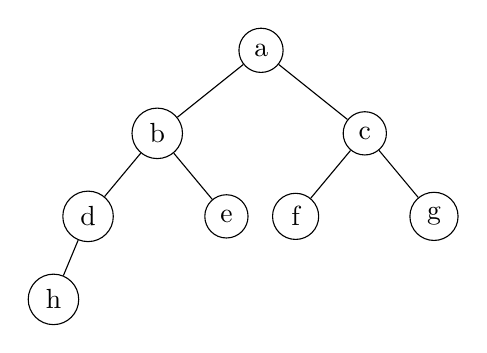
\begin{tikzpicture}[level distance=30pt,
      every node/.style={,circle,draw},
      level 1/.style={sibling distance=75pt},
      level 2/.style={sibling distance=50pt},
      level 3/.style={sibling distance=25pt}]
      \node{a}
      child{
        node{b}
        child{
          node{d}
          child{
            node{h}
          }
          child{
            edge from parent[draw=none]
          }
        }
        child{
          node{e}
        }
      }
      child{
        node{c}
        child{
          node{f}
        }
        child{
          node{g}
        }
      };
\end{tikzpicture}

Has the same time complexity of:

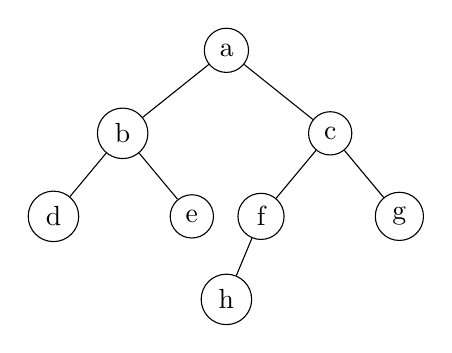
\begin{tikzpicture}[level distance=30pt,
      every node/.style={,circle,draw},
      level 1/.style={sibling distance=75pt},
      level 2/.style={sibling distance=50pt},
      level 3/.style={sibling distance=25pt}]
      \node{a}
      child{
        node{b}
        child{
          node{d}
        }
        child{
          node{e}
        }
      }
      child{
        node{c}
        child{
          node{f}
          child{
            node{h}
          }
          child{
            edge from parent[draw=none]
          }
        }
        child{
          node{g}
        }
      };
\end{tikzpicture}

Both of these have a time complexity of $\Omega(\log n)$ and $O(\log n)$. Since the $\Omega$ and $O$ time complexities are the same we can also say time complexity is $\Theta(\log n)$
\end{enumerate}

%%%%%%%%%%%%%%%%%%%%%%%%%%%%%%%%%%%%%%%%%%%%%%%%%%%%%%%%%%%%%
\subsection{[8+4 marks]}
\begin{enumerate}[(a)]
\item Beginning with an empty AVL tree, insert the keys 4, 0, 8, 1, 2, 3. Show the tree that
results after inserting each key.
\begin{center}
  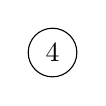
\begin{tikzpicture}[level distance=30pt,
      every node/.style={,circle,draw},
      level 1/.style={sibling distance=200pt},
      level 2/.style={sibling distance=100pt},
      level 3/.style={sibling distance=48pt},
      level 4/.style={sibling distance=30pt},
      every lower node part/.style={blue}]
    \node {4};
  \end{tikzpicture}

  \begin{tikzpicture}[level distance=30pt,
      every node/.style={,circle,draw},
      level 1/.style={sibling distance=100pt},
      every lower node part/.style={blue}]
    \node {4}
    child{
        node{0}
    }
    child {edge from parent[draw=none]}
    ;
  \end{tikzpicture}

  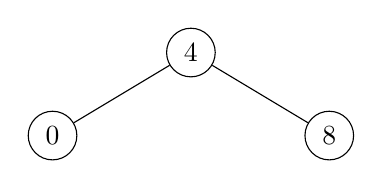
\begin{tikzpicture}[level distance=30pt,
      every node/.style={,circle,draw},
      level 1/.style={sibling distance=100pt},
      every lower node part/.style={blue}]
    \node {4}
    child{
        node{0}
    }
    child {
        node{8}
    };
  \end{tikzpicture}

  \begin{tikzpicture}[level distance=30pt,
      every node/.style={,circle,draw},
      level 1/.style={sibling distance=200pt},
      level 2/.style={sibling distance=100pt},
      every lower node part/.style={blue}]
    \node {4}
    child{
        node{0}
        child {
            edge from parent[draw=none]
        }
        child {
            node{1}
        }
    }
    child {
        node{8}
    };
  \end{tikzpicture}

  \begin{tikzpicture}[level distance=30pt,
      every node/.style={,circle,draw},
      level 1/.style={sibling distance=200pt},
      level 2/.style={sibling distance=100pt},
      level 3/.style={sibling distance=50pt},
      every lower node part/.style={blue}]
    \node {4}
    child{
        node{0}
        child {
            edge from parent[draw=none]
        }
        child {
            node{1}
            child {
                edge from parent[draw=none]
            }
            child{
                node{2}
            }
        }
    }
    child {
        node{8}
    };
  \end{tikzpicture}

  \begin{tikzpicture}[level distance=30pt,
      every node/.style={,circle,draw},
      level 1/.style={sibling distance=200pt},
      level 2/.style={sibling distance=100pt},
      level 3/.style={sibling distance=50pt},
      every lower node part/.style={blue}]
    \node {4}
    child{
        node{1}
        child {
            node{0}
        }
        child {
            node{2}
        }
    }
    child {
        node{8}
    };
  \end{tikzpicture}

  \begin{tikzpicture}[level distance=30pt,
      every node/.style={,circle,draw},
      level 1/.style={sibling distance=200pt},
      level 2/.style={sibling distance=100pt},
      level 3/.style={sibling distance=50pt},
      every lower node part/.style={blue}]
    \node {4}
    child{
        node{1}
        child {
            node{0}
        }
        child {
            node{2}
            child {
                edge from parent[draw=none]
            }
            child{
                node{3}
            }
        }
    }
    child {
        node{8}
    };
  \end{tikzpicture}


  \begin{tikzpicture}[level distance=30pt,
      every node/.style={,circle,draw},
      level 1/.style={sibling distance=200pt},
      level 2/.style={sibling distance=100pt},
      level 3/.style={sibling distance=50pt},
      every lower node part/.style={blue}]
    \node {4}
    child{
        node{2}
        child {
            node{1}
            child{
                node{0}
            }
            child {
                edge from parent[draw=none]
            }
        }
        child {
            node{3}
        }
    }
    child {
        node{8}
    };
  \end{tikzpicture}


  \begin{tikzpicture}[level distance=30pt,
      every node/.style={,circle,draw},
      level 1/.style={sibling distance=200pt},
      level 2/.style={sibling distance=100pt},
      level 3/.style={sibling distance=50pt},
      every lower node part/.style={blue}]
    \node {2}
    child{
        node{1}
        child{
            node{0}
        }
        child {
            edge from parent[draw=none]
        }
    }
    child {
        node{4}
        child{
            node{3}
        }
        child{
            node{8}
        }
    };

    \end{tikzpicture}

\end{center}

\item Delete the key 5 from the following tree using in-order predecessor for swaps. Show the AVL tree that results at each step (after or before each rotation).

\begin{center}
  \begin{tikzpicture}[level distance=30pt,
      every node/.style={,circle,draw},
      level 1/.style={sibling distance=200pt},
      level 2/.style={sibling distance=100pt},
      level 3/.style={sibling distance=48pt},
      level 4/.style={sibling distance=30pt},
      every lower node part/.style={blue}]
    \node {5}
    child {
      node {3}
      child {
        node {2}
        child {
          node {1}
        }
        child {edge from parent[draw=none]}
      }
      child {
        node {4}
      }
    }
    child {
      node {10}
      child {
        node {8}
        child {
          node {7}
          child {
            node {6}
          }
          child {edge from parent[draw=none]}
        }
        child {
          node {9}
        }
      }
      child {
        node {12}
        child {
          node {11}
        }
        child {edge from parent[draw=none]}
      }
    };
  \end{tikzpicture}

  \begin{tikzpicture}[level distance=30pt,
      every node/.style={,circle,draw},
      level 1/.style={sibling distance=200pt},
      level 2/.style={sibling distance=100pt},
      level 3/.style={sibling distance=48pt},
      level 4/.style={sibling distance=30pt},
      every lower node part/.style={blue}]
    \node {4}
    child {
      node {3}
      child {
        node {2}
        child {
          node {1}
        }
        child {edge from parent[draw=none]}
      }
      child {
        edge from parent[draw=none]
      }
    }
    child {
      node {10}
      child {
        node {8}
        child {
          node {7}
          child {
            node {6}
          }
          child {edge from parent[draw=none]}
        }
        child {
          node {9}
        }
      }
      child {
        node {12}
        child {
          node {11}
        }
        child {edge from parent[draw=none]}
      }
    };
  \end{tikzpicture}


  \begin{tikzpicture}[level distance=30pt,
      every node/.style={,circle,draw},
      level 1/.style={sibling distance=200pt},
      level 2/.style={sibling distance=100pt},
      level 3/.style={sibling distance=48pt},
      level 4/.style={sibling distance=30pt},
      every lower node part/.style={blue}]
    \node {4}
    child {
      node {2}
      child {
        node {1}
      }
      child {
        node{3}
      }
    }
    child {
      node {10}
      child {
        node {8}
        child {
          node {7}
          child {
            node {6}
          }
          child {edge from parent[draw=none]}
        }
        child {
          node {9}
        }
      }
      child {
        node {12}
        child {
          node {11}
        }
        child {edge from parent[draw=none]}
      }
    };
  \end{tikzpicture}

  \begin{tikzpicture}[level distance=30pt,
      every node/.style={,circle,draw},
      level 1/.style={sibling distance=200pt},
      level 2/.style={sibling distance=100pt},
      level 3/.style={sibling distance=48pt},
      level 4/.style={sibling distance=30pt},
      every lower node part/.style={blue}]
    \node {4}
    child {
      node {2}
      child {
        node {1}
      }
      child {
        node{3}
      }
    }
    child {
      node {8}
      child {
          node {7}
          child {
            node {6}
          }
          child {edge from parent[draw=none]}
      }
      child {
        node{10}
        child{
            node {12}
            child {
              node {11}
            }
            child {edge from parent[draw=none]}
          }
        child{
            node{9}
        }
        }
    };
  \end{tikzpicture}


  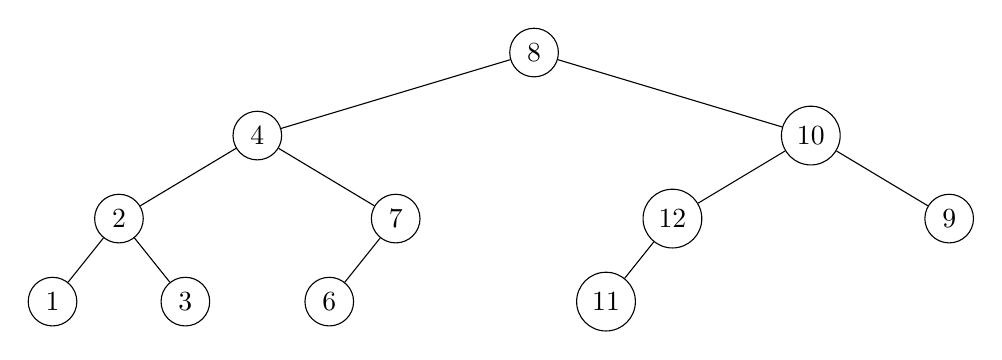
\begin{tikzpicture}[level distance=30pt,
      every node/.style={,circle,draw},
      level 1/.style={sibling distance=200pt},
      level 2/.style={sibling distance=100pt},
      level 3/.style={sibling distance=48pt},
      level 4/.style={sibling distance=30pt},
      every lower node part/.style={blue}]
    \node{8}
    child {
        node{4}
        child {
            node {2}
            child {
                node {1}
            }
            child {
                node{3}
            }
        }
        child{
            node {7}
            child {
                node {6}
            }
            child {
                edge from parent[draw=none]
            }
        }
    }
    child {
        node{10}
        child{
            node {12}
            child {
              node {11}
            }
            child {
                edge from parent[draw=none]
            }
        }
        child{
            node{9}
        }
    };
  \end{tikzpicture}




\end{center}

\end{enumerate}

%%%%%%%%%%%%%%%%%%%%%%%%%%%%%%%%%%%%%%%%%%%%%%%%%%%%%%%%%%%%%
\subsection{[7+4 marks]}
\begin{enumerate}[(a)]
\item Beginning with an empty 2-3 tree, insert the keys 3, 0, 8, 4, 1, 5, 2. Show the tree that results after inserting each key.

\begin{center}
  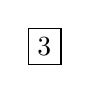
\begin{tikzpicture}
    \tikzstyle{bplus}=[rectangle split, rectangle split horizontal,rectangle split ignore empty parts,draw]
    \tikzstyle{every node}=[bplus]
    \tikzstyle{level 1}=[sibling distance=60mm]
    \tikzstyle{level 2}=[sibling distance=15mm]
      \node{3}
      ;
  \end{tikzpicture}

  \begin{tikzpicture}
    \tikzstyle{bplus}=[rectangle split, rectangle split horizontal,rectangle split ignore empty parts,draw]
    \tikzstyle{every node}=[bplus]
    \tikzstyle{level 1}=[sibling distance=60mm]
    \tikzstyle{level 2}=[sibling distance=15mm]
    \node{3}
    child{
      node{0}
    }
    child {
      edge from parent[draw=none]
    }
    ;
  \end{tikzpicture}

  \begin{tikzpicture}
    \tikzstyle{bplus}=[rectangle split, rectangle split horizontal,rectangle split ignore empty parts,draw]
    \tikzstyle{every node}=[bplus]
    \tikzstyle{level 1}=[sibling distance=60mm]
    \tikzstyle{level 2}=[sibling distance=15mm]
    \node{3}
    child{
      node{0}
    }
    child {
      node{8}
    }
    ;
  \end{tikzpicture}

  \begin{tikzpicture}
    \tikzstyle{bplus}=[rectangle split, rectangle split horizontal,rectangle split ignore empty parts,draw]
    \tikzstyle{every node}=[bplus]
    \tikzstyle{level 1}=[sibling distance=60mm]
    \tikzstyle{level 2}=[sibling distance=15mm]
    \node{3}
    child{
      node{0}
    }
    child {
      node{4 \nodepart{two} 8}
    }
    ;
  \end{tikzpicture}

  \begin{tikzpicture}
    \tikzstyle{bplus}=[rectangle split, rectangle split horizontal,rectangle split ignore empty parts,draw]
    \tikzstyle{every node}=[bplus]
    \tikzstyle{level 1}=[sibling distance=60mm]
    \tikzstyle{level 2}=[sibling distance=15mm]
    \node{3}
    child{
      node{0 \nodepart{two} 1}
    }
    child {
      node{4 \nodepart{two} 8}
    }
    ;
  \end{tikzpicture}

  \begin{tikzpicture}
    \tikzstyle{bplus}=[rectangle split, rectangle split horizontal,rectangle split ignore empty parts,draw]
    \tikzstyle{every node}=[bplus]
    \tikzstyle{level 1}=[sibling distance=40mm]
    \tikzstyle{level 2}=[sibling distance=15mm]
    \node{3 \nodepart{two} 5}
    child{
      node{0 \nodepart{two} 1}
    }
    child{
      node{4}
    }
    child{
      node{8}
    }
    ;
  \end{tikzpicture}

  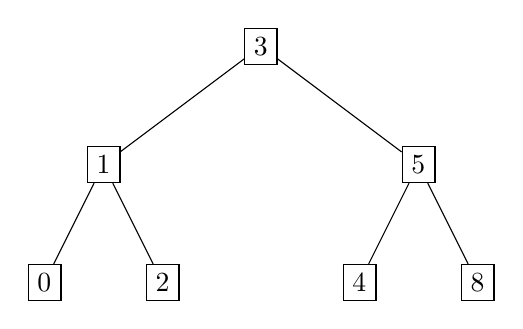
\begin{tikzpicture}
    \tikzstyle{bplus}=[rectangle split, rectangle split horizontal,rectangle split ignore empty parts,draw]
    \tikzstyle{every node}=[bplus]
    \tikzstyle{level 1}=[sibling distance=40mm]
    \tikzstyle{level 2}=[sibling distance=15mm]
    \node{3}
    child{
      node{1}
      child{
        node{0}
      }
      child{
        node{2}
      }
    }
    child{
      node{5}
      child{
        node{4}
      }
      child{
        node{8}
      }
    }
    ;
  \end{tikzpicture}

\end{center}
\item Delete the key 3 from your answer to part (a), replacing it with its in-order successor and show the 2-3 tree that results.
\begin{center}
  \begin{tikzpicture}
    \tikzstyle{bplus}=[rectangle split, rectangle split horizontal,rectangle split ignore empty parts,draw]
    \tikzstyle{every node}=[bplus]
    \tikzstyle{level 1}=[sibling distance=40mm]
    \tikzstyle{level 2}=[sibling distance=15mm]
    \node{1 \nodepart{two} 4}
    child{
      node{0}
    }
    child {
      node{2}
    }
    child{
      node{5 \nodepart{two} 8}
    }
    ;
  \end{tikzpicture}

\end{center}


\end{enumerate}

%%%%%%%%%%%%%%%%%%%%%%%%%%%%%%%%%%%%%%%%%%%%%%%%%%%%%%%%%%%%%
\subsection{[8 marks]}
Consider a variant of AVL trees that uses size instead of height as balancing parameter.
Each node has a leftDescendants, a rightDescendants and a balance field containing the number of descendants in each of the subtrees as well as the balance defined as the ratio between the left and right subtree sizes, i.e.
    \[
     balance = (rightDescendants+1) / (leftDescendants+1).
     \]
The idea now is that a tree is ``balanced'' if the left and right sides are within a multiplicative factor of two of each other, i.e $1/2 \leq balance \leq 2$.

\begin{enumerate}[(a)]
\item Prove that balanced trees have height $\Theta(\log n)$ where $n$ is the number of keys in the tree.

Looking at the two children of the parent node, in the worst case you have a smaller subtree and a larger subtree where the larger subtree has twice as many nodes as the smaller subtree. So:

\begin{align*}
    2n_{smaller} + 2 &= n_{larger}+1\\
    n-1 &= 3 n_{smaller} +2\\
    \intertext{Since the smaller subtree is a subtree of height h-1 we can switch it to N(h-1) where N is the minimum number of nodes required to make a tree of height h-1}
    n - 3 &= 3N(h-1)\\
    &= 3N(h-1)\\
    &= 3^2 N(h-2)\\
    &= \dots\\
    &= 3^h \\
    h &= \log_3(n-3)\\
    &< \log_3(n)\\
    &< \frac{\log n}{\log 3}\\
    &< c\log n\\
    &\in O(\log n)
\end{align*}

Looking at the two children of the parent node, in the best case you have two equal subtrees. So:

\begin{align*}
  n_{a} + n_{b}+1  &= n \\
  2n_a + 1 &= n\\
  n &> 2n_a\\
  \intertext{Since $n_a$ is the number of nodes in a subtree of height h-1 we can sub in N(h-1)}
  n &> 2N(h-1)\\
  & \dots\\
  &> 2^h\\
  h< \log n
  &\in\Omega(\log n)
\end{align*}

Since $O(\log n)$ and $\Omega(\log n)$, the time complexity is $\Theta(\log n)$.
\end{enumerate}

%%%%%%%%%%%%%%%%%%%%%%%%%%%%%%%%%%%%%%%%%%%%%%%%%%%%%%%%%%%%%
\subsection{[9 marks]}
Suppose the leaf pages in extendible hashing can hold at most 3 keys. Show the result after keys with the following hash values are inserted in this order:

00001, 10000, 10001, 00011, 01111, 00000, 11010, 11111, 10111.

You need only show the extendible has table after either a local or global depth value changes.
Also show the final extendible hash table.

\begin{center}
    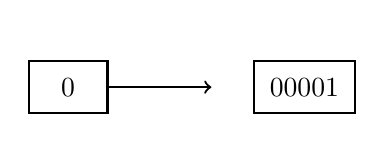
\begin{tikzpicture}[
      grow=right,
      level 1/.style={sibling distance=2cm,level distance=3cm},
      edge from parent/.style={draw=none},
      pointer/.style={thick, shorten >=5pt, ->,draw=black},
      dpointer/.style={thick, shorten >=15pt, ->,draw=black},
      every label/.style={font=\footnotesize,draw=none},
      every node/.style={rectangle,thick,draw=black, text ragged, inner sep=2mm,minimum width=10mm}
      ]
      \node[label=,rectangle split, rectangle split parts=1] (directory) {
        \nodepart{one} 0
      }
        child {
          \block{1}{1}{a}{ 00001 }
        };
      \path(directory.one east) edge [dpointer] (a.west);
    \end{tikzpicture}

    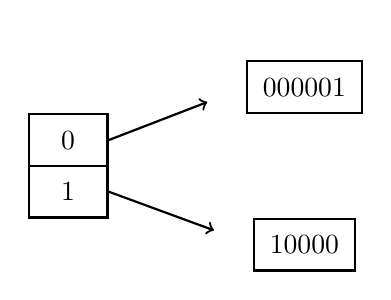
\begin{tikzpicture}[
      grow=right,
      level 1/.style={sibling distance=2cm,level distance=3cm},
      edge from parent/.style={draw=none},
      pointer/.style={thick, shorten >=5pt, ->,draw=black},
      dpointer/.style={thick, shorten >=15pt, ->,draw=black},
      every label/.style={font=\footnotesize,draw=none},
      every node/.style={rectangle,thick,draw=black, text ragged, inner sep=2mm,minimum width=10mm}
      ]
      \node[label=,rectangle split, rectangle split parts=2] (directory) {
        \nodepart{one} 0
        \nodepart{two} 1
      }
        child {
          \block{1}{1}{b}{ 10000 }
        }
        child{
          \block{1}{1}{a} { 000001 }
        };
      \path(directory.one east) edge [dpointer] (a.west);
      \path(directory.two east) edge [dpointer] (b.west);
    \end{tikzpicture}

    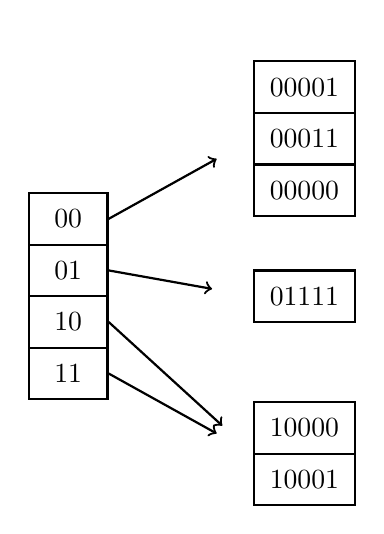
\begin{tikzpicture}[
      grow=right,
      level 1/.style={sibling distance=2cm,level distance=3cm},
      edge from parent/.style={draw=none},
      pointer/.style={thick, shorten >=5pt, ->,draw=black},
      dpointer/.style={thick, shorten >=15pt, ->,draw=black},
      every label/.style={font=\footnotesize,draw=none},
      every node/.style={rectangle,thick,draw=black, text ragged, inner sep=2mm,minimum width=10mm}
      ]
      \node[label=,rectangle split, rectangle split parts=4] (directory) {
        \nodepart{one} 00
        \nodepart{two} 01
        \nodepart{three} 10
        \nodepart{four} 11
      }
        child{
          \block{1}{2}{c}{ 10000 \nodepart{second} 10001}
        }
        child {
          \block{1}{1}{b}{ 01111 }
        }
        child{
          \block{1}{3}{a} { 00001 \nodepart{second} 00011 \nodepart{third} 00000 }
        };
      \path(directory.one east) edge [dpointer] (a.west);
      \path(directory.two east) edge [dpointer] (b.west);
      \path(directory.three east) edge [dpointer] (c.west);
      \path(directory.four east) edge [dpointer] (c.west);
    \end{tikzpicture}

    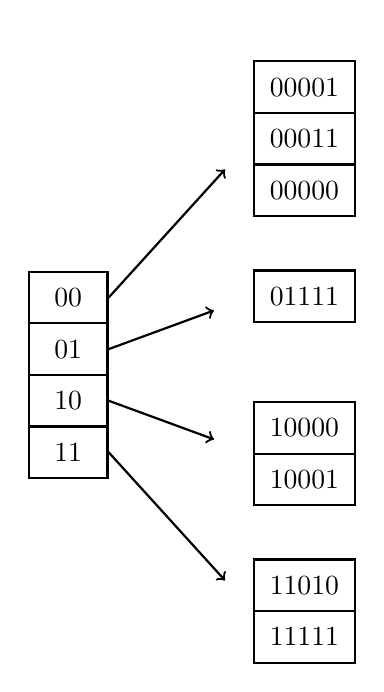
\begin{tikzpicture}[
      grow=right,
      level 1/.style={sibling distance=2cm,level distance=3cm},
      edge from parent/.style={draw=none},
      pointer/.style={thick, shorten >=5pt, ->,draw=black},
      dpointer/.style={thick, shorten >=15pt, ->,draw=black},
      every label/.style={font=\footnotesize,draw=none},
      every node/.style={rectangle,thick,draw=black, text ragged, inner sep=2mm,minimum width=10mm}
      ]
      \node[label=,rectangle split, rectangle split parts=4] (directory) {
        \nodepart{one} 00
        \nodepart{two} 01
        \nodepart{three} 10
        \nodepart{four} 11
      }
        child {
          \block{1}{2}{d}{ 11010 \nodepart{second} 11111}
        }
        child{
          \block{1}{2}{c}{ 10000 \nodepart{second} 10001}
        }
        child {
          \block{1}{1}{b}{ 01111 }
        }
        child{
          \block{1}{3}{a} { 00001 \nodepart{second} 00011 \nodepart{third} 00000 }
        };
      \path(directory.one east) edge [dpointer] (a.west);
      \path(directory.two east) edge [dpointer] (b.west);
      \path(directory.three east) edge [dpointer] (c.west);
      \path(directory.four east) edge [dpointer] (d.west);
    \end{tikzpicture}

    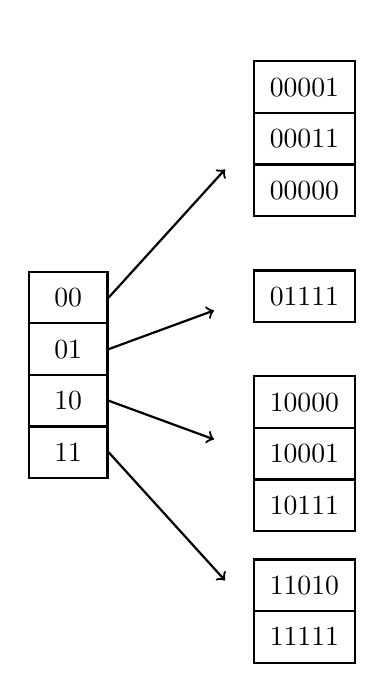
\begin{tikzpicture}[
      grow=right,
      level 1/.style={sibling distance=2cm,level distance=3cm},
      edge from parent/.style={draw=none},
      pointer/.style={thick, shorten >=5pt, ->,draw=black},
      dpointer/.style={thick, shorten >=15pt, ->,draw=black},
      every label/.style={font=\footnotesize,draw=none},
      every node/.style={rectangle,thick,draw=black, text ragged, inner sep=2mm,minimum width=10mm}
      ]
      \node[label=,rectangle split, rectangle split parts=4] (directory) {
        \nodepart{one} 00
        \nodepart{two} 01
        \nodepart{three} 10
        \nodepart{four} 11
      }
        child {
          \block{1}{2}{d}{ 11010 \nodepart{second} 11111 }
        }
        child {
          \block{1}{3}{c}{ 10000 \nodepart{second} 10001 \nodepart{third} 10111}
        }
        child {
          \block{1}{1}{b}{ 01111 }
        }
        child {
          \block{1}{3}{a}{ 00001 \nodepart{second} 00011 \nodepart{third} 00000 }
        };
      \path(directory.one east) edge [dpointer] (a.west);
      \path(directory.two east) edge [dpointer] (b.west);
      \path(directory.three east) edge [dpointer] (c.west);
      \path(directory.four east) edge [dpointer] (d.west);
    \end{tikzpicture}



  \end{center}






\end{document}
